\documentclass[rascunho,xindy]{Classe-Latex-FEI/fei}
\usepackage[utf8]{inputenc}
\usepackage{xcolor,colortbl}

\graphicspath{{images/}}

\author{Nome do Autor}
\title{Título do Trabalho}
\subtitulo{subtítulo}

%\cidade{Cidade}
\instituicao{Centro Universitário da FEI - Fundação Educacional Inaciana Pe. Saboia de Medeiros}

\makeindex

\begin{document}

\maketitle


\begin{resumo}
Resumo do Projeto, preferencialmente em no máximo uma folha. Deve iniciar com uma breve introdução do assunto contextualizando-o, apresentar o objetivo, a metodologia de maneira concisa, mostrando de forma sistema o que e como será feito e os resultados esperados, enfocando as contribuições do trabalho.
\palavraschave{Palavras. Chave. Vão. Aqui.}
\end{resumo}


% \listoffigures
% \listoftables
% \listofalgorithms
% \glsaddall
% \printglossaries
\tableofcontents

\chapter{Introdução}

A Introdução serve para apresentar o assunto em seu contexto geral, apresentando os principais conceitos que o avaliador irá necessitar para entender a proposta, além de situar a proposta no contexto do ambiente científico do Brasil e do Mundo. Pode estender-se por 3 a 4 páginas.

\chapter{Objetivos}

O item objetivos apresenta a proposta de trabalho. Ou seja, de maneira clara e concisa o que pretende-se realizar. O que será desenvolvido, medido, qual coleta de dados, e/ou experimento que será executado de maneira a envolver seres humanos. Deve ser descrito em um ou dois parágrafos.

\chapter{Metodologia}

\section{Voluntários}

Este item deve conter a descrição da ou das amostras de voluntários que serão necessárias para a realização da pesquisa. Qual o número de amostras, o número de voluntários por amostra e total, de que forma e de onde serão selecionados, quais as características específicas de inclusão e/ou exclusão desses voluntários.

Exemplo:

"Serão selecionados, dentro da comunidade acadêmica, 50 voluntários não portadores de deficiência física ou motora com idades entre 20 e 30 anos que serão brevemente entrevistados sobre a existência de algum histórico anterior de lesões, queixa de dores ou qualquer comprometimento neuromuscular nos membros superiores e inferiores. Não havendo qualquer uma das condições acima, os voluntários estarão aptos a participar dos ensaios e, após a leitura do termo de consentimento livre e esclarecido, será necessário que o assinem caso estejam de acordo."

\section{Procedimentos experimentais}

Este item deve descrever a metodologia, as etapas que devem ser cumpridas para a execução do experimento em si.

Exemplo:

"O procedimento de teste será realizado em duas sessões. Na primeira sessão, o voluntário será esclarecido sobre o protocolo experimental e serão coletadas medidas como altura, peso corporal, e comprimentos do braço, antebraço, pernas e tronco. Ainda nessa sessão, o voluntário se familiarizará com o sistema e com os movimentos a serem realizados, bem como as condições propostas para as avaliações.

Na segunda sessão, a ser realizada no mesmo dia da primeira sessão, colocaremos alguns sensores autoadesivos sobre a pele do voluntário (eletrodos de superfície). Estes sensores detectam a ativação muscular, ou seja, o sinal mioelétrico e serão colados no seu braço, antebraço, ombro, tórax (peito).

A cinemática dos membros superiores em todos os testes será medida por meio de 2 unidades inerciais, uma afixada no antebraço e uma no braço, ambas fixadas na porção média dos segmentos e alinhadas com as respectivas direções longitudinais.  O sistema é composto de sensores inerciais para análise de movimento humano 3D e substitui um sistema de câmeras, que, apesar de ser mais usual para avaliações cinemáticas, é muito mais caro e não permitiria que os dados fossem recolhidos fora de um laboratório. 

Com relação à medição do esforço muscular durante a realização dos movimentos, serão monitorados a contribuição dos músculos envolvidos (Fig. \ref{fig:corpo_humano}) por meio de eletromiografia. Na Fig. \ref{fig:corpo_humano}, os dois pontos amarelos nos músculos indicam a orientação do eletrodo em relação à direção das fibras musculares, conforme manual da NORAXON \cite{konradabc}. Estes são músculos envolvidos na extensão do punho e flexão e extensão do ombro e do cotovelo, movimentos estes preponderantes durante o processo de interesse.

\begin{figure}[!htb]
\centering
\caption{Posições anatômicas de localização de eletrodos, vista frontal e dorsal. \cite{konradabc}}
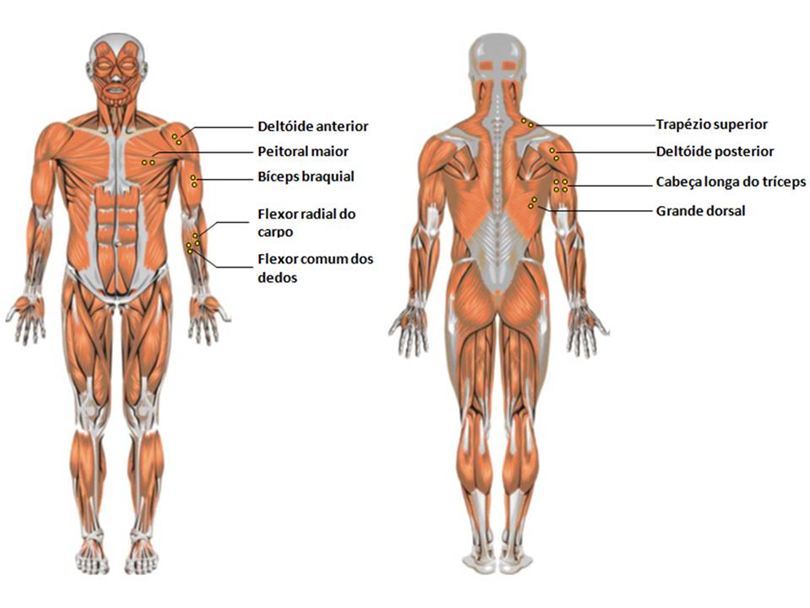
\includegraphics[scale=1.0]{corpo_humano}
\label{fig:corpo_humano}
\end{figure}

Após a colocação dos sensores citados, será solicitado ao voluntário que se sente no banco para um teste de força máxima. Neste teste, o voluntário será instruído a aplicar sua força máxima à manopla. Nestas condições, serão obtidos os valores correspondentes à contração isométrica voluntária máxima (MVIC) dos músculos envolvidos, considerando o valor médio de 3 aquisições para cada posição da alavanca comentado anteriormente."

\section{Dados experimentais coletados}

Em todos os ensaios, serão coletados dados de eletromiografia (sEMG) e de cinemática dos membros superiores. Serão coletadas também, os dados de forças aplicadas na manopla, nas três direções (tangencial, radial e transversal) por meio de um equipamento de aquisição da Ricardo.

Para a aquisição do sEMG será utilizado um Sistema de Eletromiografia wireless de 16 canais da Noraxon, denominado Telemyo DTS Desk Receiver W/16 Channels \& MR3 Master Software. Os eletrodos a serem utilizados são de superfície, de Ag.AgCl, autoadesivos com gel. O padrão de colocação e posicionamento, bem como o equipamento, seguem as recomendações da SENIAM.

\section{Processamento e análise de dados coletados}

Neste item, as técnicas de processamento dos dados devem ser descritas. Ou seja, o que será feito com os dados após a sua aquisição, até se atingir o objetivo proposto?

Exemplo:

O sinal de sEMG deve ser amplificado e filtrado por um passa faixas de 20 – 500Hz. Após o processo de suavização, segue-se com a normalização pelo MVIC. A frequência de aquisição mínima a ser programada no sistema deve ser 1000 Hz.

Um programa escrito em Matlab será utilizado para retificar os resultados, fazer a separação por grupo muscular, calcular o RMS (Root Mean Square) tanto do teste MVIC quanto os ensaios em condições normais do experimento dinâmico e comparar os valores de EMG obtidos entre todos os voluntários.

Por fim, os dados de sEMG de cada músculo analisado, de força na manopla da alavanca e de momentos articulares estimados serão comparados para quantificar o esforço realizado em cada troca de marcha e comparado à percepção de cada voluntário.

\chapter{Riscos}

Os riscos são mínimos não havendo nenhuma evidência específica de que o participante irá sofrer algum dano como consequência imediata ou tardia do estudo. Em função do esforço realizado durante as repetições dos movimentos, poderá haver um desconforto devido a uma leve fadiga muscular nos braços e ombros. Contudo, como forma de evitar será utilizado um período de descanso durante o ensaio caso.

\chapter{Cronograma de Execução}

\begin{table}[ht]
  \caption{Cronograma de trabalho}
  \begin{center}
      \begin{tabular}{|l |l |l |l |l ||l |l |l |l ||l |l |l |l |}
      \hline
      % \T and \B would not work if it is placed here (needs to go inside cell)
      Ano        & \multicolumn{4}{c||}{Ano 1} & \multicolumn{4}{c||}{Ano 2} & \multicolumn{4}{c|}{Ano 3} \\
      \hline
      Trimestre & T1 & T2 & T3 & T4 & T1 & T2 & T3 & T4 & T1 & T2 & T3 & T4 \\
      \hline
      Submissão do protocolo            & \cellcolor{black!80} & \cellcolor{black!80} & \cellcolor{black!80} & \cellcolor{black!80} &   &   &   &   &   &   &   &   \\
      Pesquisa bibliográfica            & \cellcolor{black!80} & \cellcolor{black!80} & \cellcolor{black!80} & \cellcolor{black!80} &   &   &   &   &   &   &   &   \\
      Seleção de grupo de voluntários   &   & \cellcolor{black!80} & \cellcolor{black!80} & \cellcolor{black!80} & \cellcolor{black!80} &   &   &   &   &   &   &   \\
      Realização de coleta de dados     &   &   &   & \cellcolor{black!80} & \cellcolor{black!80} & \cellcolor{black!80} &   &   &   &   &   &   \\
      Relatório Parcial                 &   &   &   & \cellcolor{black!80} & \cellcolor{black!80} & \cellcolor{black!80} & \cellcolor{black!80} &   &   &   &   &   \\
      Avaliação de resultados           &   &   &   &   & \cellcolor{black!80} & \cellcolor{black!80} & \cellcolor{black!80} & \cellcolor{black!80} & \cellcolor{black!80} &   &   &   \\ 
      Publicação                        &   &   &   &   &   & \cellcolor{black!80} & \cellcolor{black!80} & \cellcolor{black!80} & \cellcolor{black!80} &   &   &   \\
      Participação em congresssos       &   &   &   &   &   &   &   &   & \cellcolor{black!80} & \cellcolor{black!80} &   &   \\
      \hline
      Relatório Final                   &   & \cellcolor{black!80} & \cellcolor{black!80} & \cellcolor{black!80} & \cellcolor{black!80} & \cellcolor{black!80} & \cellcolor{black!80} & \cellcolor{black!80} & \cellcolor{black!80} & \cellcolor{black!80} & \cellcolor{black!80} & \cellcolor{black!80} \\
      \hline
      \end{tabular}
  \end{center}
  \label{table:cronograma}
\end{table} 

Duração: 24 meses.

\chapter{Financiamento}

Este projeto está sendo financiado pela própria instituição. Não há financiamento específico de modo que não estamos apresentando nenhuma planilha de custos. A presente pesquisa está sendo desenvolvida segundo recursos de uso corrente na instituição, sem nenhuma alocação específica. Ou seja, para o desenvolvimento do estudo, hora submetido à apreciação do comitê de ética, não há alocação específica de recursos; por este motivo não está sendo apresentado nenhuma planilha.

\chapter{Equipe Executora}

\begin{tabular}{| r || l |}
    \hline
        Nome:   & aluno \\ \hline
        CPF:    & XXX.XXX.XXX-X \\ \hline
        Lattes: & endereço do link \\ \hline
    \hline
        Nome:   & outro aluno e/ou professor participante \\ \hline
        CPF:    & XXX.XXX.XXX-X \\ \hline
        Lattes: & endereço do link \\ \hline
    \hline
        Nome:   & Maria Claudia Ferrari de Castro \\ \hline
        CPF:    & 104.951.588-95 \\ \hline
        Lattes: & http://lattes.cnpq.br/7429780004238103 \\
    \hline
\end{tabular}

\bibliography{projeto-comite-etica}

\end{document}
